% FIGURE 1 - LENGTH SCALES IN ATMOSPHERIC SCIENCES

\begin{figure}
\centering
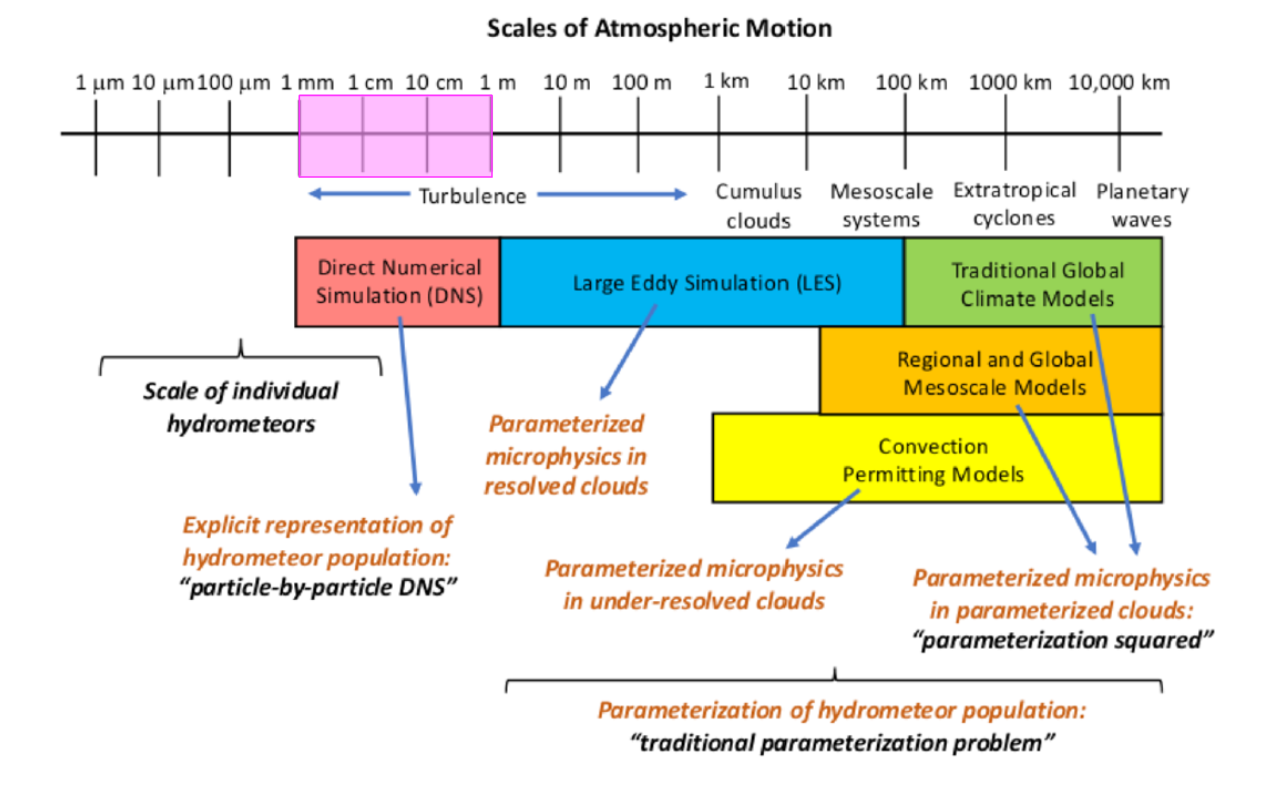
\includegraphics[width=13cm]{figures/0-01_atmo-scales.png}
\caption{
Hierarchy of atmospheric models and the scales of atmospheric motion reproduced from \textcite{Morrison2020} with author's permission.
Coloured rectangles represent types of simulations commonly used when working with respective length scales, and comments emphasise transition from directly resolving most elements of the model (left) to including more and more parameterisations with the increase of scale (right).
Magenta rectangle positioned on the axis was added to emphasise range of scales that corresponds to simulations discussed in this thesis.}
\label{fig:atmo-scales}
\end{figure}